\subsection{External Interface Requirements}

\subsection{Functional Requirements}

\subsubsection{Mapping on requirements}

\subsubsection{Use case diagrams}

\subsubsection{Use cases}

\subsubsection*{  UC1. Unregistered user signs up}

\begin{table}[H]
   \begin{tabularx}{\textwidth}{|p{3cm}|X|}
   \hline
   \textbf{Actor} & Unregistered user \\ \hline
   \textbf{Entry conditions} & User is on login page of BBP \\ \hline
   \textbf{Event flow} & 
   1. User clicks to register on BBP \newline 
   2. BBP asks user to insert his informations for the account \newline
   3. User inserts his informations \newline
   4. BBP validates the inserted personal informations \newline
   5. BBP sends the registration outcome 
   \\ \hline
   \textbf{Exit conditions} & An account is created \\ \hline
   \textbf{Exceptions} & Username already taken \newline Password not valid \newline Connection error while registering \\ \hline
   \end{tabularx}
\end{table}

\begin{figure}[H]
    \centering
    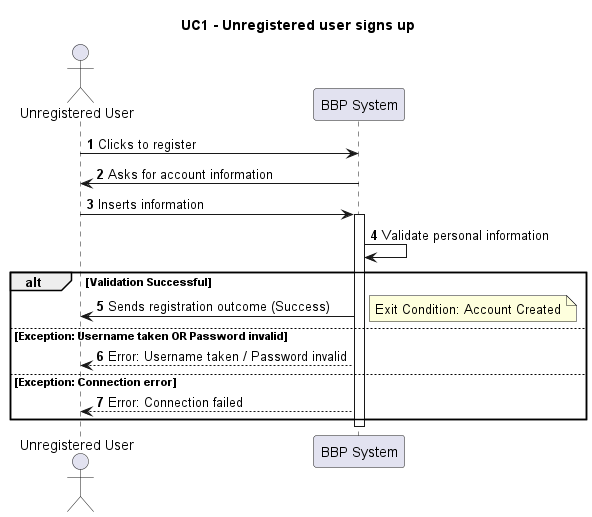
\includegraphics[width=0.9\textwidth]{./out/RASD/uml/UC1/UC1_SignUp.png}
    \caption{Use Case Diagram for UC1: Unregistered user signs up}
\end{figure}

\subsubsection*{  UC2. User logs in the account}

\begin{table}[H]
   \begin{tabularx}{\textwidth}{|p{3cm}|X|}
   \hline
   \textbf{Actor} & Registered user \\ \hline
   \textbf{Entry conditions} & Unregistered is on login page of BBP \\ \hline
   \textbf{Event flow} & 
   1. User clicks to login on BBP \newline
   2. BBP asks user to insert username and password of the account he wants to log in \newline
   3. User inserts his username \newline
   4. BBP validates the inserted username and password \newline
   5. BBP sends login outcome
   \\ \hline
   \textbf{Exit conditions} & User logs BBP system \\ \hline
   \textbf{Exceptions} & Inserted username not existent \newline Wrong inserted password for specified username \newline Connection error while logging in \\ \hline
   \end{tabularx}
\end{table}

\begin{figure}[H]
    \centering
    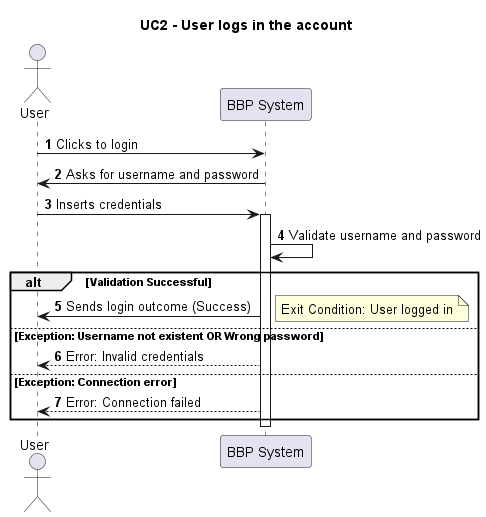
\includegraphics[width=0.9\textwidth]{./out/RASD/uml/UC2/UC2_Login.png}
    \caption{Use Case Diagram for UC2: User logs in the account}
\end{figure}

\subsubsection*{  UC3. User manually adds bike trip}

\begin{table}[H]
   \begin{tabularx}{\textwidth}{|p{3cm}|X|}
   \hline
   \textbf{Actor} & Registered user \\ \hline
   \textbf{Entry conditions} & User is registered and logged in \newline User is on "New trip" page \\ \hline
   \textbf{Event flow} &
   1. User clicks on "Insert a bike trip" button \newline
   2. BBP asks to insert a name for the trip \newline
   3. User inserts name of the trip \newline
   4. BBP validates inserted name \newline
   5. User inserts traveled roads \newline
   6. BBP calculate and returns the complete traveled route \newline
   7. User confirms calculated route \newline
   8. User inserted optional information, i.e obstacles \newline
   9. BBP calculates status based on inserted informations and shows to user \newline
   10. User clicks "Save trip" button \newline
   11. BBP saves trip, and informs user of outcome
   \\ \hline
   \textbf{Exit conditions} & Inserted trip is saved \\ \hline
   \textbf{Exceptions} & BBP can't calculate a route based on inserted roads \newline User already saved a route with the same name \\ \hline
   \end{tabularx}
\end{table}

\begin{figure}[H]
    \centering
    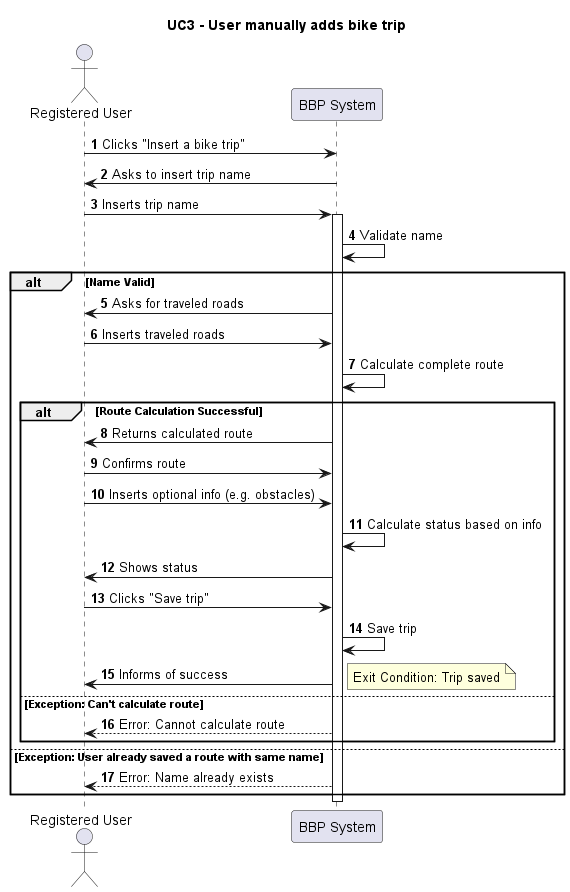
\includegraphics[width=0.9\textwidth]{./out/RASD/uml/UC3/UC3_ManualAdd.png}
    \caption{Use Case Diagram for UC3: User manually adds bike trip}
\end{figure}

\subsubsection*{  UC4. User automatically records bike trip}

\begin{table}[H]
   \begin{tabularx}{\textwidth}{|p{3cm}|X|}
   \hline
   \textbf{Actor} & Registered user \\ \hline
   \textbf{Entry conditions} & User is registered and logged in \newline User is on "New trip" page \\ \hline
   \textbf{Event flow} &
   1. User clicks to start automatic recording mode \newline
   2. BBP starts taking data from user's phone GPS \newline
   3. BBP recognize user is cycling, based on his velocity from sensors \newline
   4. BBP traces position and encountered obstacles with user's phone sensors and GPS \newline
   5. BBP recognize user stopped cycling \newline
   6. User finished automatic recording \newline
   7. BBP asks user to confirm or correct recorded data \newline
   8. User optionally corrects data and click confirm \newline
   9. BBP calculate status based on recorded and inserted data and shows to user \newline
   10. User insert a name for the trip and clicks "Save trip" button \newline
   11. BBP saves trip, and informs user of outcome
   \\ \hline
   \textbf{Exit conditions} & Recorded trip is saved \\ \hline
   \textbf{Exceptions} & GPS signal lost \newline Sensor permissions negated \newline User already saved a route with the same name \newline User discards recorded trip \\ \hline
   \end{tabularx}
\end{table}

\begin{figure}[H]
    \centering
    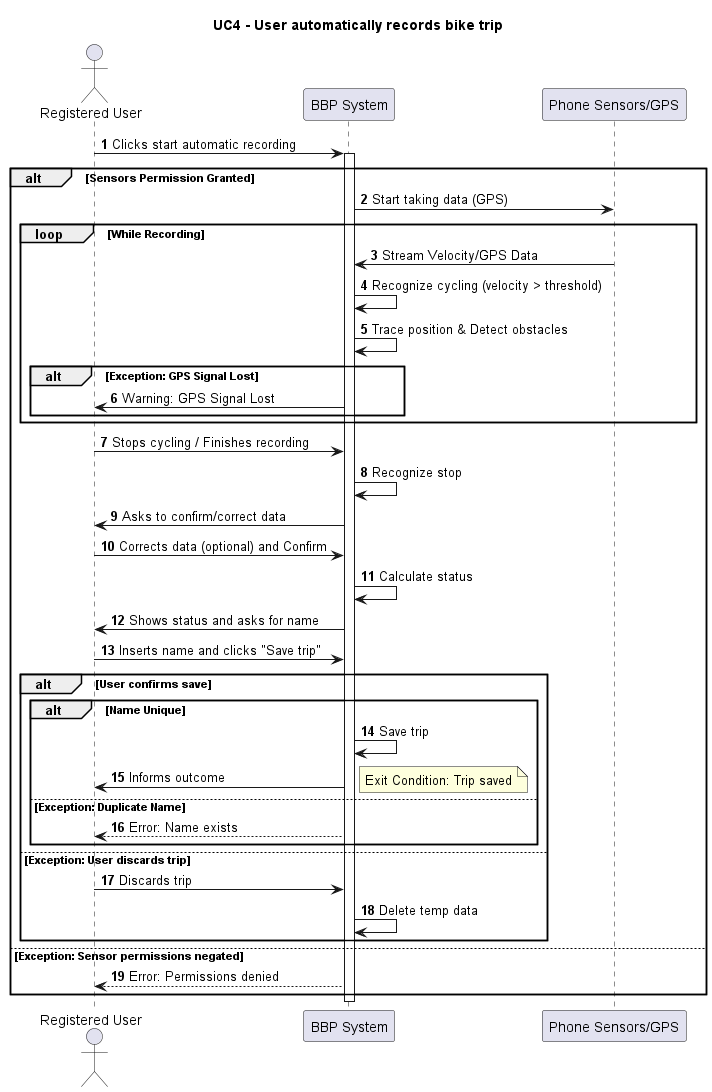
\includegraphics[width=0.9\textwidth]{./out/RASD/uml/UC4/UC4_AutoRecord.png}
    \caption{Use Case Diagram for UC4: User automatically records bike trip}
\end{figure}

\subsubsection*{  UC5. User views his bike trip history}

\begin{table}[H]
   \begin{tabular}{|p{3cm}|p{12cm}|}
   \hline
   \textbf{Actor} & Registered user \\ \hline
   \textbf{Entry conditions} & 
   User is registered and logged in \newline
   User is on "Your trips" page \\ \hline
   \textbf{Event flow} &
   1. User opens on "Bike trip history" section \newline
   2. BBP loads history of trips of user \newline
   3. User visualizes his trips
   \\ \hline
   \textbf{Exit conditions} & User closes "Bike trip history" section \\ \hline
   \textbf{Exceptions} & User does not have any saved trips \\ \hline
   \end{tabular}
\end{table}

\begin{figure}[H]
    \centering
    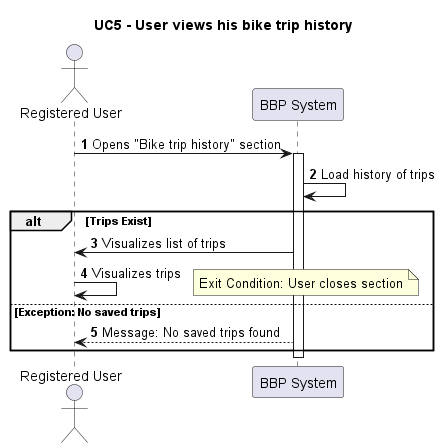
\includegraphics[width=0.9\textwidth]{./out/RASD/uml/UC5/UC5_ViewHistory.png}
    \caption{Use Case Diagram for UC5: User views his bike trip history}
\end{figure}

\subsubsection*{  UC6. User views his bike trip statistics}

\begin{table}[H]
   \begin{tabular}{|p{3cm}|p{12cm}|}
   \hline
   \textbf{Actor} & Registered user \\ \hline
   \textbf{Entry conditions} & 
   User is registered and logged in \newline
   User selected a specific trip from history \\ \hline
   \textbf{Event flow} &
   1. User clicks on "View statistics" button \newline
   2. BBP loads complessive statistics of traveled bike trips, and statistics for each trip \newline
   3. User clicks on a specific trip \newline
   4. BBP visualizes in-depth statistics for that trip
   \\ \hline
   \textbf{Exit conditions} & User closes "Trips Statistics" section \\ \hline
   \textbf{Exceptions} & User does not have any trip to calculate statistics on \\ \hline
   \end{tabular}
\end{table}

\begin{figure}[H]
    \centering
    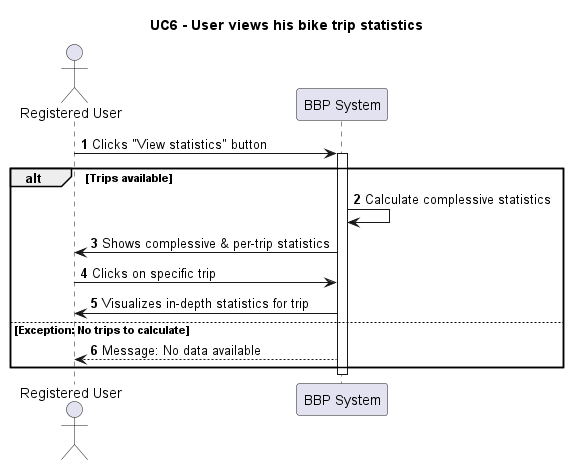
\includegraphics[width=0.9\textwidth]{./out/RASD/uml/UC6/UC6_ViewStats.png}
    \caption{Use Case Diagram for UC6: User views his bike trip statistics}
\end{figure}

\subsubsection*{  UC7. User publishes recorded trip}

\begin{table}[H]
   \begin{tabular}{|p{3cm}|p{12cm}|}
   \hline
   \textbf{Actor} & Registered user \\ \hline
   \textbf{Entry conditions} & 
   User is registered and logged in \newline
   User selected a specific trip from history \\ \hline
   \textbf{Event flow} &
   1. User click on "Publish trip" \newline
   2. BBP ask confirm to user if information are correct and if he is sure to make the trip public \newline
   3. User confirms the intention to publish \newline
   4. BBP publishes the trip, making it visible to all users
   \\ \hline
   \textbf{Exit conditions} & User's trip is published and visible by all users \\ \hline
   \textbf{Exceptions} & Connection error while publishing \\ \hline
   \end{tabular}
\end{table}

\begin{figure}[H]
    \centering
    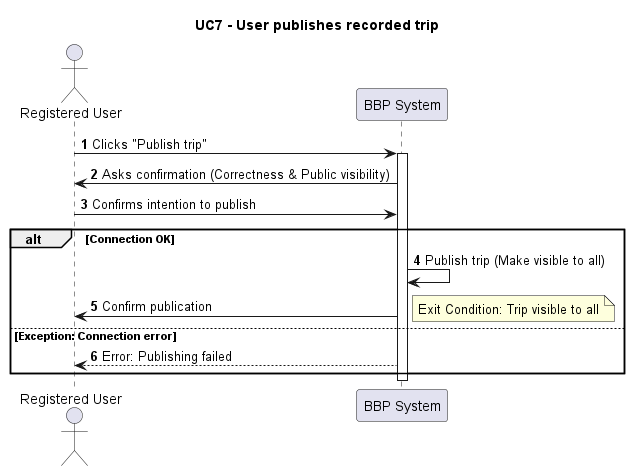
\includegraphics[width=0.9\textwidth]{./out/RASD/uml/UC7/UC7_PublishTrip.png}
    \caption{Use Case Diagram for UC7: User publishes recorded trip}
\end{figure}

\subsubsection*{  UC8. User modify one of his saved trips}

\begin{table}[H]
   \begin{tabular}{|p{3cm}|p{12cm}|}
   \hline
   \textbf{Actor} & Registered user \\ \hline
   \textbf{Entry conditions} & 
   User is registered and logged in \newline
   User selected a specific trip from history \\ \hline
   \textbf{Event flow} &
   1. User click on "Modify trip" \newline
   2. BBP allows users to modify saved data about trip \newline
   3. User modifies trip data \newline
   4. BBP validate changes of trip data \newline
   5. User confirm the changes of trip data \newline
   6. BBP modifies trip data on database and if the trip is public propagates changes for every user
   \\ \hline
   \textbf{Exit conditions} & Trip data is modified \\ \hline
   \textbf{Exceptions} & Inserted data is not valid \newline Connection error while propagating changes of public trip\\ \hline
   \end{tabular}
\end{table}

\begin{figure}[H]
    \centering
    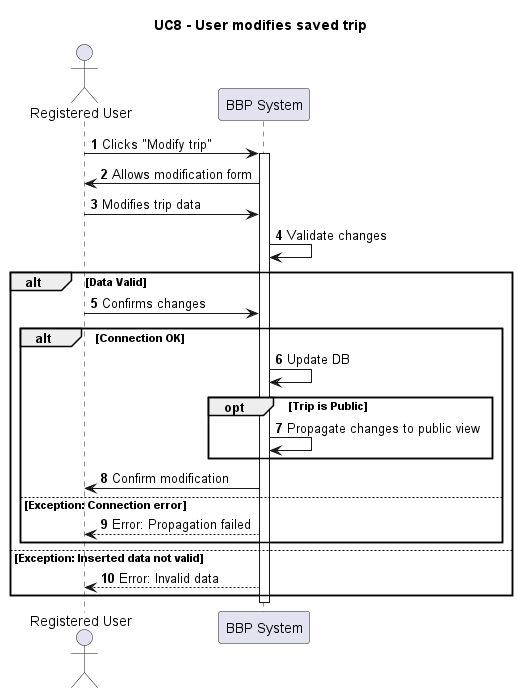
\includegraphics[width=0.9\textwidth]{./out/RASD/uml/UC8/UC8_ModifyTrip.png}
    \caption{Use Case Diagram for UC8: User modifies one of his saved trips}
\end{figure}

\subsubsection*{  UC9. User views possible bike routes on map}

\begin{table}[H]
   \begin{tabular}{|p{3cm}|p{12cm}|}
   \hline
   \textbf{Actor} & Registered user \newline Unregistered user \\ \hline
   \textbf{Entry conditions} & 
   User is on "Path search" section \\ \hline
   \textbf{Event flow} &
   1. BBP asks user to insert start and end point of route \newline
   2. User inserts start and end point \newline
   3. BBP visualizes every routes, with related score, between selected points
   \\ \hline
   \textbf{Exit conditions} & Paths are visualized \\ \hline
   \textbf{Exceptions} & Mapping service unavailable \newline Connection error while retrieving paths \newline No route found between the selected points \\ \hline
   \end{tabular}
\end{table}

\begin{figure}[H]
    \centering
    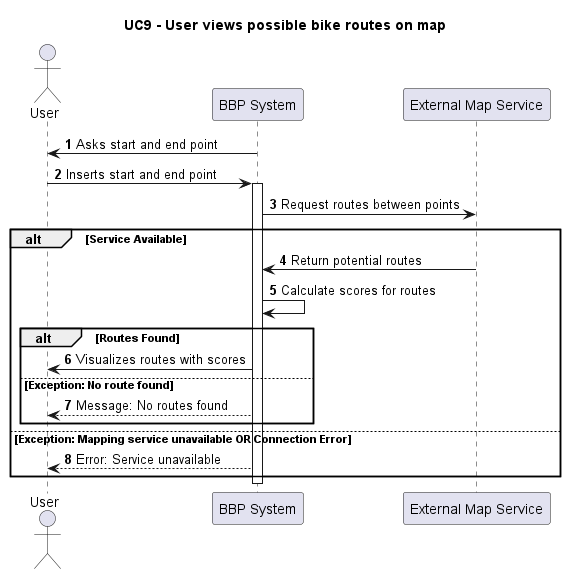
\includegraphics[width=0.9\textwidth]{./out/RASD/uml/UC9/UC9_ViewMapRoutes.png}
    \caption{Use Case Diagram for UC9: User views possible bike routes on map}
\end{figure}

\subsubsection*{  UC10. User views additional information about selected path on map}

\begin{table}[H]
   \begin{tabular}{|p{3cm}|p{12cm}|}
   \hline
   \textbf{Actor} & Registered user \newline Unregistered user \\ \hline
   \textbf{Entry conditions} & 
   User is on "Path search" section visualizing paths between 2 points \\ \hline
   \textbf{Event flow} &
   1. User clicks on a specific path on the map \newline
   2. BBP shows details about trip, i.e statistics, distance, obstacles etc..
   \\ \hline
   \textbf{Exit conditions} & Additionals informations of a trip are visualized \\ \hline
   \textbf{Exceptions} \\ \hline
   \end{tabular}
\end{table}

\begin{figure}[H]
    \centering
    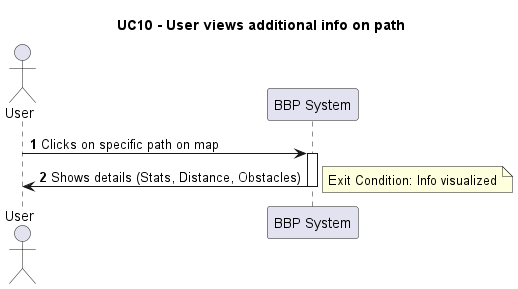
\includegraphics[width=0.9\textwidth]{./out/RASD/uml/UC10/UC10_ViewPathDetails.png}
    \caption{Use Case Diagram for UC10: User views additional information about selected path on map}
\end{figure}

\subsubsection*{  UC11. User start navigation on selected bike path}

\begin{table}[H]
   \begin{tabular}{|p{3cm}|p{12cm}|}
   \hline
   \textbf{Actor} & Registered user \newline Unregistered user \\ \hline
   \textbf{Entry conditions} & 
   User selected a path on the map \\ \hline
   \textbf{Event flow} &
   1. User click to open route on a third-party mapping service \newline
   2. BBP opens third-party mapping service, giving it coordinates of start and end point
   \\ \hline
   \textbf{Exit conditions} & Additionals informations of a trip are visualized \\ \hline
   \textbf{Exceptions} & hird-party mapping service not available\\ \hline
   \end{tabular}
\end{table}

\begin{figure}[H]
    \centering
    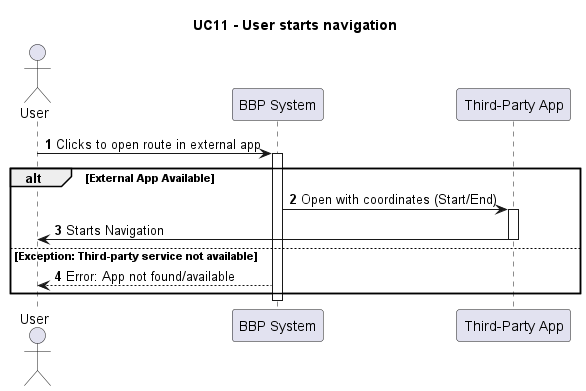
\includegraphics[width=0.9\textwidth]{./out/RASD/uml/UC11/UC11_StartNav.png}
    \caption{Use Case Diagram for UC11: User start navigation on selected bike path}
\end{figure}

\subsubsection*{  UC12. User modifies profile data}

\begin{table}[H]
   \begin{tabular}{|p{3cm}|p{12cm}|}
   \hline
   \textbf{Actor} & Registered user \\ \hline
   \textbf{Entry conditions} & 
   User is registered and logged in \newline
   User is on profile page of BPP \\ \hline
   \textbf{Event flow} &
   1. User clicks on modify profile data \newline
   2. User insert new personal data \newline
   3. BBP validates new personal data \newline
   4. User confirms changes on personal data \newline
   5. BBP update user personal data
   \\ \hline
   \textbf{Exit conditions} & User personal data are modified \\ \hline
   \textbf{Exceptions} & New username already taken \newline New password not valid \newline Connection error while modifying profile data \\ \hline
   \end{tabular}
\end{table}

\begin{figure}[H]
    \centering
    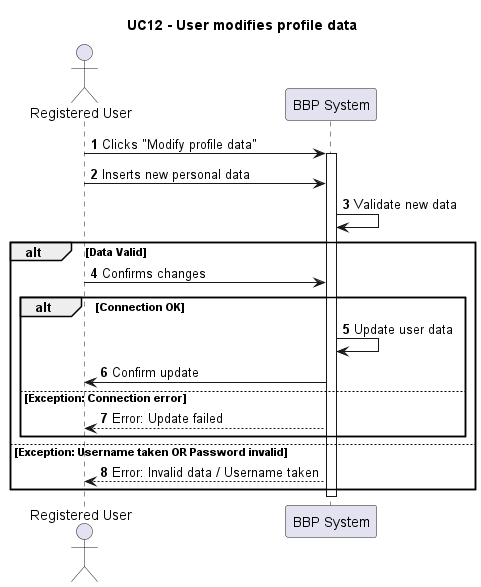
\includegraphics[width=0.9\textwidth]{./out/RASD/uml/UC12/UC12_ModifyProfile.png}
    \caption{Use Case Diagram for UC12: User modifies profile data}
\end{figure}

\subsubsection*{  UC13. User logs out the account}

\begin{table}[H]
   \begin{tabular}{|p{3cm}|p{12cm}|}
   \hline
   \textbf{Actor} & Registered user \\ \hline
   \textbf{Entry conditions} & 
   User is registered and logged in \\ \hline
   \textbf{Event flow} &
   1. User clicks on log out button \newline
   2. BBP terminate access of user on the account \newline
   3. BBP returns user to log in page
   \\ \hline
   \textbf{Exit conditions} & User is disconnected from the account \\ \hline
   \textbf{Exceptions} \\ \hline
   \end{tabular}
\end{table}

\begin{figure}[H]
    \centering
    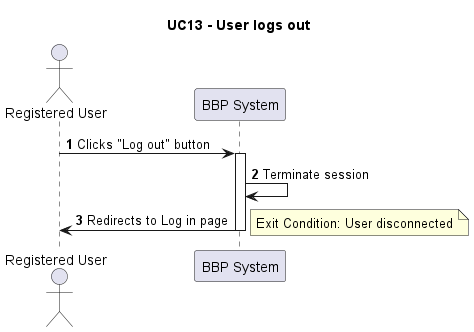
\includegraphics[width=0.9\textwidth]{./out/RASD/uml/UC13/UC13_Logout.png}
    \caption{Use Case Diagram for UC13: User logs out the account}
\end{figure}